%% ------------- Portuguese version ------------
% \documentclass{sbrt}
% \usepackage[english,brazil]{babel}
% \usepackage[utf8]{inputenc}
% \newtheorem{theorem}{Teorema}
%% ------------------------------------
%% If writing in English, remove the lines above
%% and uncomment the lines below

%% ------------- English version ---------------
\documentclass[english]{sbrt}
\usepackage[english]{babel}
\usepackage[utf8]{inputenc}
\usepackage{cite}
\usepackage{graphicx}
\usepackage{float}
\usepackage[top=2cm,left=2cm,right=3cm,bottom=3cm]{geometry}
\usepackage{titlesec}
\usepackage[center]{caption}
\newtheorem{theorem}{Theorem}
%% ---------------------------------------------

\titlespacing*{\section}
  {0pt}{18pt}{18pt}
  
\titlespacing*{\subsection}
  {0pt}{18pt}{18pt}

\begin{document}

\title{Use case of the websocket protocol in a multiplayer browser-based game}

\author{Tiago da Silva Guerreiro and Lucas Costa dos Prazeres
  \thanks{Special thanks to professor Eduardo Cerqueira, ITEC, UFPA, Belém-PA, e-mail: cerqueira@ufpa.br}
}

\maketitle

\baselineskip = 18pt


\begin{abstract}
  Web applications have become more popular in the recent years, due to the emergence of modern programming languages and frameworks, which allows software developers to create more robust projects, in terms of performance and reliability.
  Such scenario has led to the popularization of many computer network applications that require intense real-time communication between servers and clients, like multiplayer videogames, and the creation of technologies to meet those requirements (i.e. websockets).
  This research aims to analyze websocket traffic in a simple multiplayer game, capturing its traffic using Wireshark.
  % which is the perfect oportunity to understand why would a developer or software engineer prefer to use a realtime communitation
  % protocol on a real project, instead of the simple HTTP request/response.
  Moreover, we also present a small experiment intended to show how the packet drop parameter of websocket connections behaves in a few different scenarios.

\end{abstract}
\begin{keywords}
  websocket, nodejs, multiplayer game, TCP, real-time
\end{keywords}

\section{\textbf{Introduction}}

%The web has never been more close to our daily lives than nowadays. 
The internet is a vital component of the society, being present in every aspect of daily life.
Everyday, lots of web applications are designed and developed for
many use cases. Some of them need to be fast and able to update their state constantly, such as currency platforms, multimedia chats and multiplayer games~\cite{chen2011framework}\cite{kawase2015development}.
This situation has drawn developers' attention to modern programming platforms and frameworks, including node.js and its ecossystem.

Node.js is not a programming language itself, but an asynchonous JavaScript runtime made to support this language on server-side applications, since JavaScript could
only be executed by browsers on web clients. Besides, node.js offers many native libraries for various purposes, including useful community-made tools. One of such libraries is socket.io, a toolset for easily handling websockets, which was released right after node.js.

Socket.io uses the websocket protocol to provide real-time and bi-directional communication between hosts (full-duplex)~\cite{zhao2013real}. Its connection mainentance behavior made possible to create applications in which the clients need to be updated as soon as some information changes on the server side. That said, this research aims to analyze websocket traffic in a simple multiplayer game. This content is expected to provide a good understanding of how the different network
actors interact with each other, and also to provide an introduction to the websocket protocol. Also, the network traffic generated by the game will be analyzed
using the Wireshark tool to compare the packet drop observed in a websocket connection, in two different scenarios.

This article is organized as follows: Section 2 introduces related works. Section 3 explains the game architecture. Section 4 presents the results obtained, and Section 5 concludes the paper.

\section{\textbf{The websocket protocol}}
The websocket protocol was first created to enable two-way communication between server and client, without the need to open multiple HTTP connections~\cite{yassein2016application}. Before the creation of this protocol, it was required to overload the HTTP protocol to poll for updates, which used different TCP connections each time and caused a high overhead. Websocket resolves this matter by enabling a single TCP connection for traffic in both directions, and mantaining the connection open to avoid unnecessary handshakes. The security of the communication is guaranteed by a key, cryptographed using SHA-1 encryption, that is passed in the header of the communication. If a message with a non-matching key arrives, the connection is closed immediately. Websocket protocol also keeps track of changes in the data, and notifies the client as soon as the data is available. The websocket protocol is well-designed for applications that need low latency to work properly, like multiplayer videogames~\cite{tai2019development}, multimedia chats and currency platforms.

\section{\textbf{The Game}}
The game is a simple web and multiplayer version of the classic snake game, in which a player needs to
catch as many fruits as possible to earn more points.

\begin{figure}[H]
  \centering
  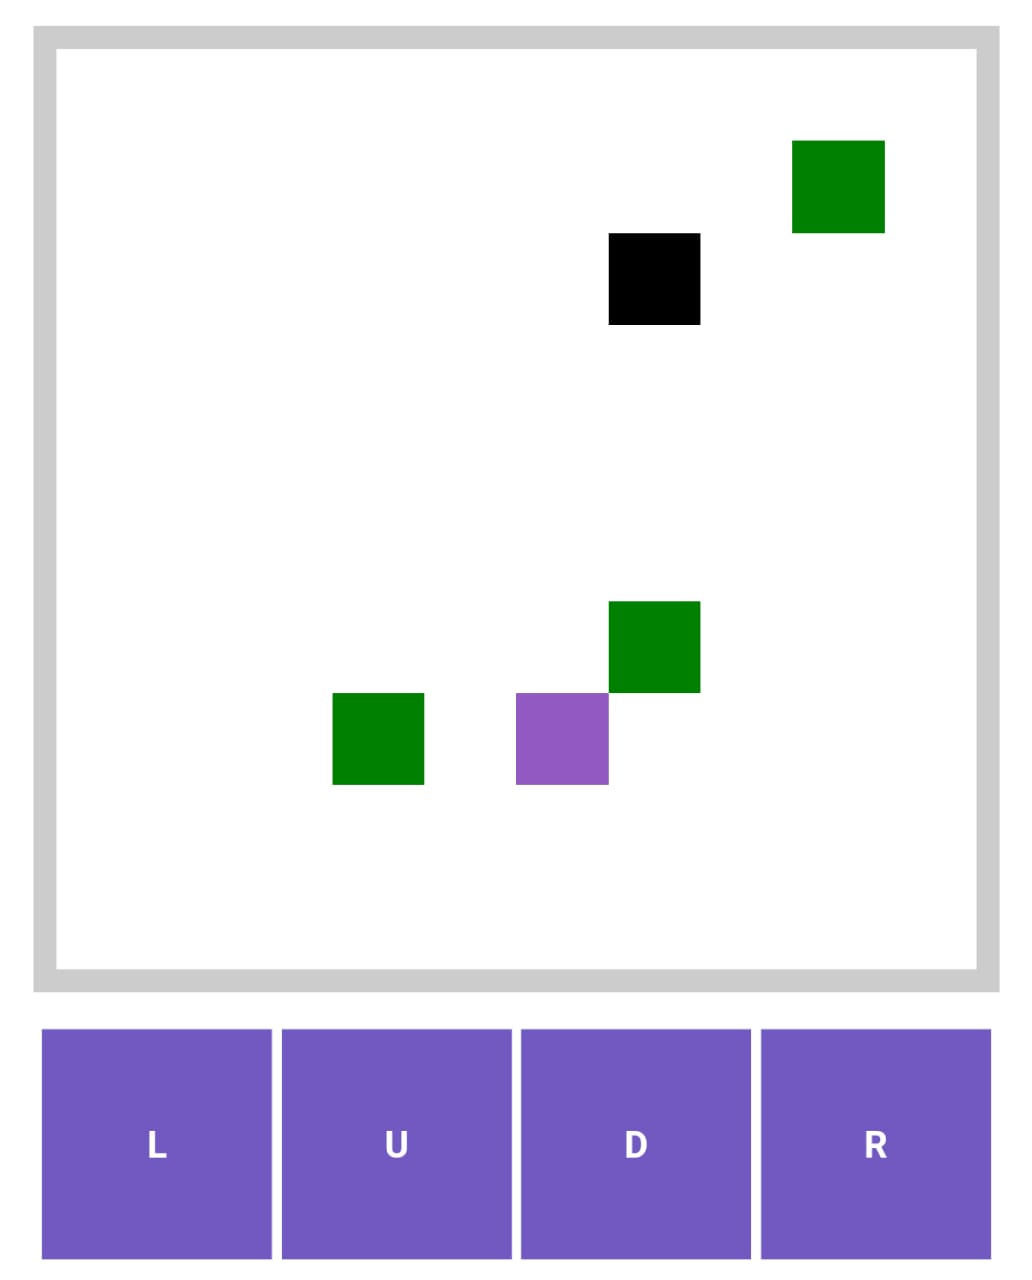
\includegraphics[width=5cm]{game-screen.jpg}
  \caption{Gameplay with 2 players and 3 fruits available}
  \label{game-screen}
\end{figure}

This project is composed by a few javascript files containing the main logic and network settings, besides an HTML with embed JavaScript with the game interface and client-side code. The backend was designed using Node.js, while the client code gets executed by the player's browser. It has a well-defined architecture, as shown on Figure~\ref{game-layers}.

\begin{figure}[H]
  \centering
  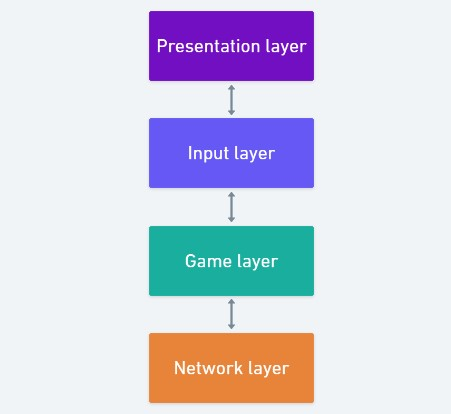
\includegraphics[width=8cm]{game-layers.jpg}
  \caption{Game architecture}
  \label{game-layers}
\end{figure}

The first layer from top to bottom is the presentation layer, which contains the HTML responsible for rendering the page, and also the required definitions for the other modules to work.
The following layer is the input layer, which handles the user inputs and propagates them to next layer. The third layer is the game layer, composed by the game logic and rules
applied to all its players, also being responsible for interpreting the commands sent by the input listenter layer above. At this level, the game state is represented as a data structure containing
all player and fruit abstractions, which are manipulated locally, propagated to the server, and then to the other clients. The last one is the network layer, in which is possible to see the actual communication logic.
Now, its important to understand how the game is setted up and how the hosts interact with each other.

\begin{figure}[H]
  \centering
  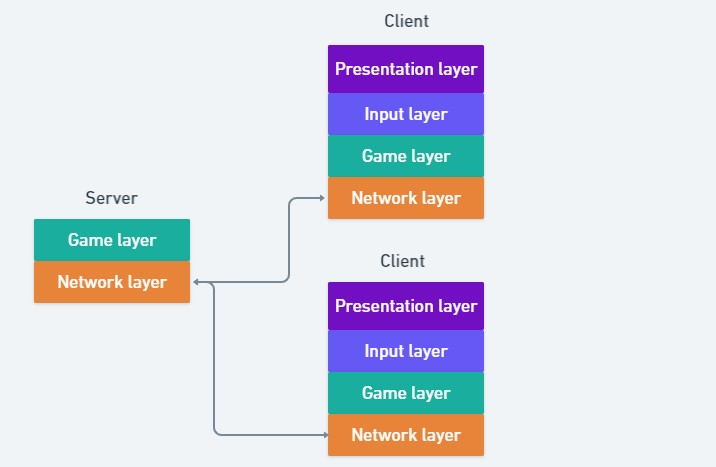
\includegraphics[width=10cm]{game-diagram.jpg}
  \caption{Interaction between server and client}
  \label{game-diagram}
\end{figure}

As shown in Figure~\ref{game-diagram}, the game consists of a server and a few clients. When the server is executed, it uses the game layer to create its own game state and the Node.js libraries "express" and "socket.io" to create a web server and a websocket server, both listening on port 3000.
Then, the client request the game page via regular HTTP request, which is reponded with the game HTML file and its javascript dependencies. After the clients receive the page, a websocket connection is started and the first message from server to the client contains the current
game state data structure, which is used by the client side to render the game screen. Meawhile, on the server side, a new websocket connection is registered and an "add-player" message its propagated to all the previously connected clients and also changes the game state on the server.
Every time a player moves, leaves the page or triggers another kind of event, its own game state is updated and a notification is sent to the server, which is responsible for syncronizing all players states by notifying them as well.

\section{\textbf{IO analysis}}

Besides having the hosts comunicating with each other, it is important to understand the quality of this connection.
Since this is a simple game, the authors intended to keep this analysis as much straightforward as possible, looking at a
single quality of service parameter which impacts directly the experience from the players: the Input-Output (IO) statiscs. The simplicity mentioned before was
also applied to the experiment itself, consisting of two nodes, a game server and a client (a smartphone), connected through a local wifi using a single router. The whole websocket
traffic was captured in a packet sniffing tool called \textit{Wireshark}, running on the server, on two different situations: first, both client and server were close to the router, then the hosts and the router
were separeted by a physical barrier. This experiment captured a 60 second match, including the whole communication cycle.

\begin{figure}[H]
  \centering
  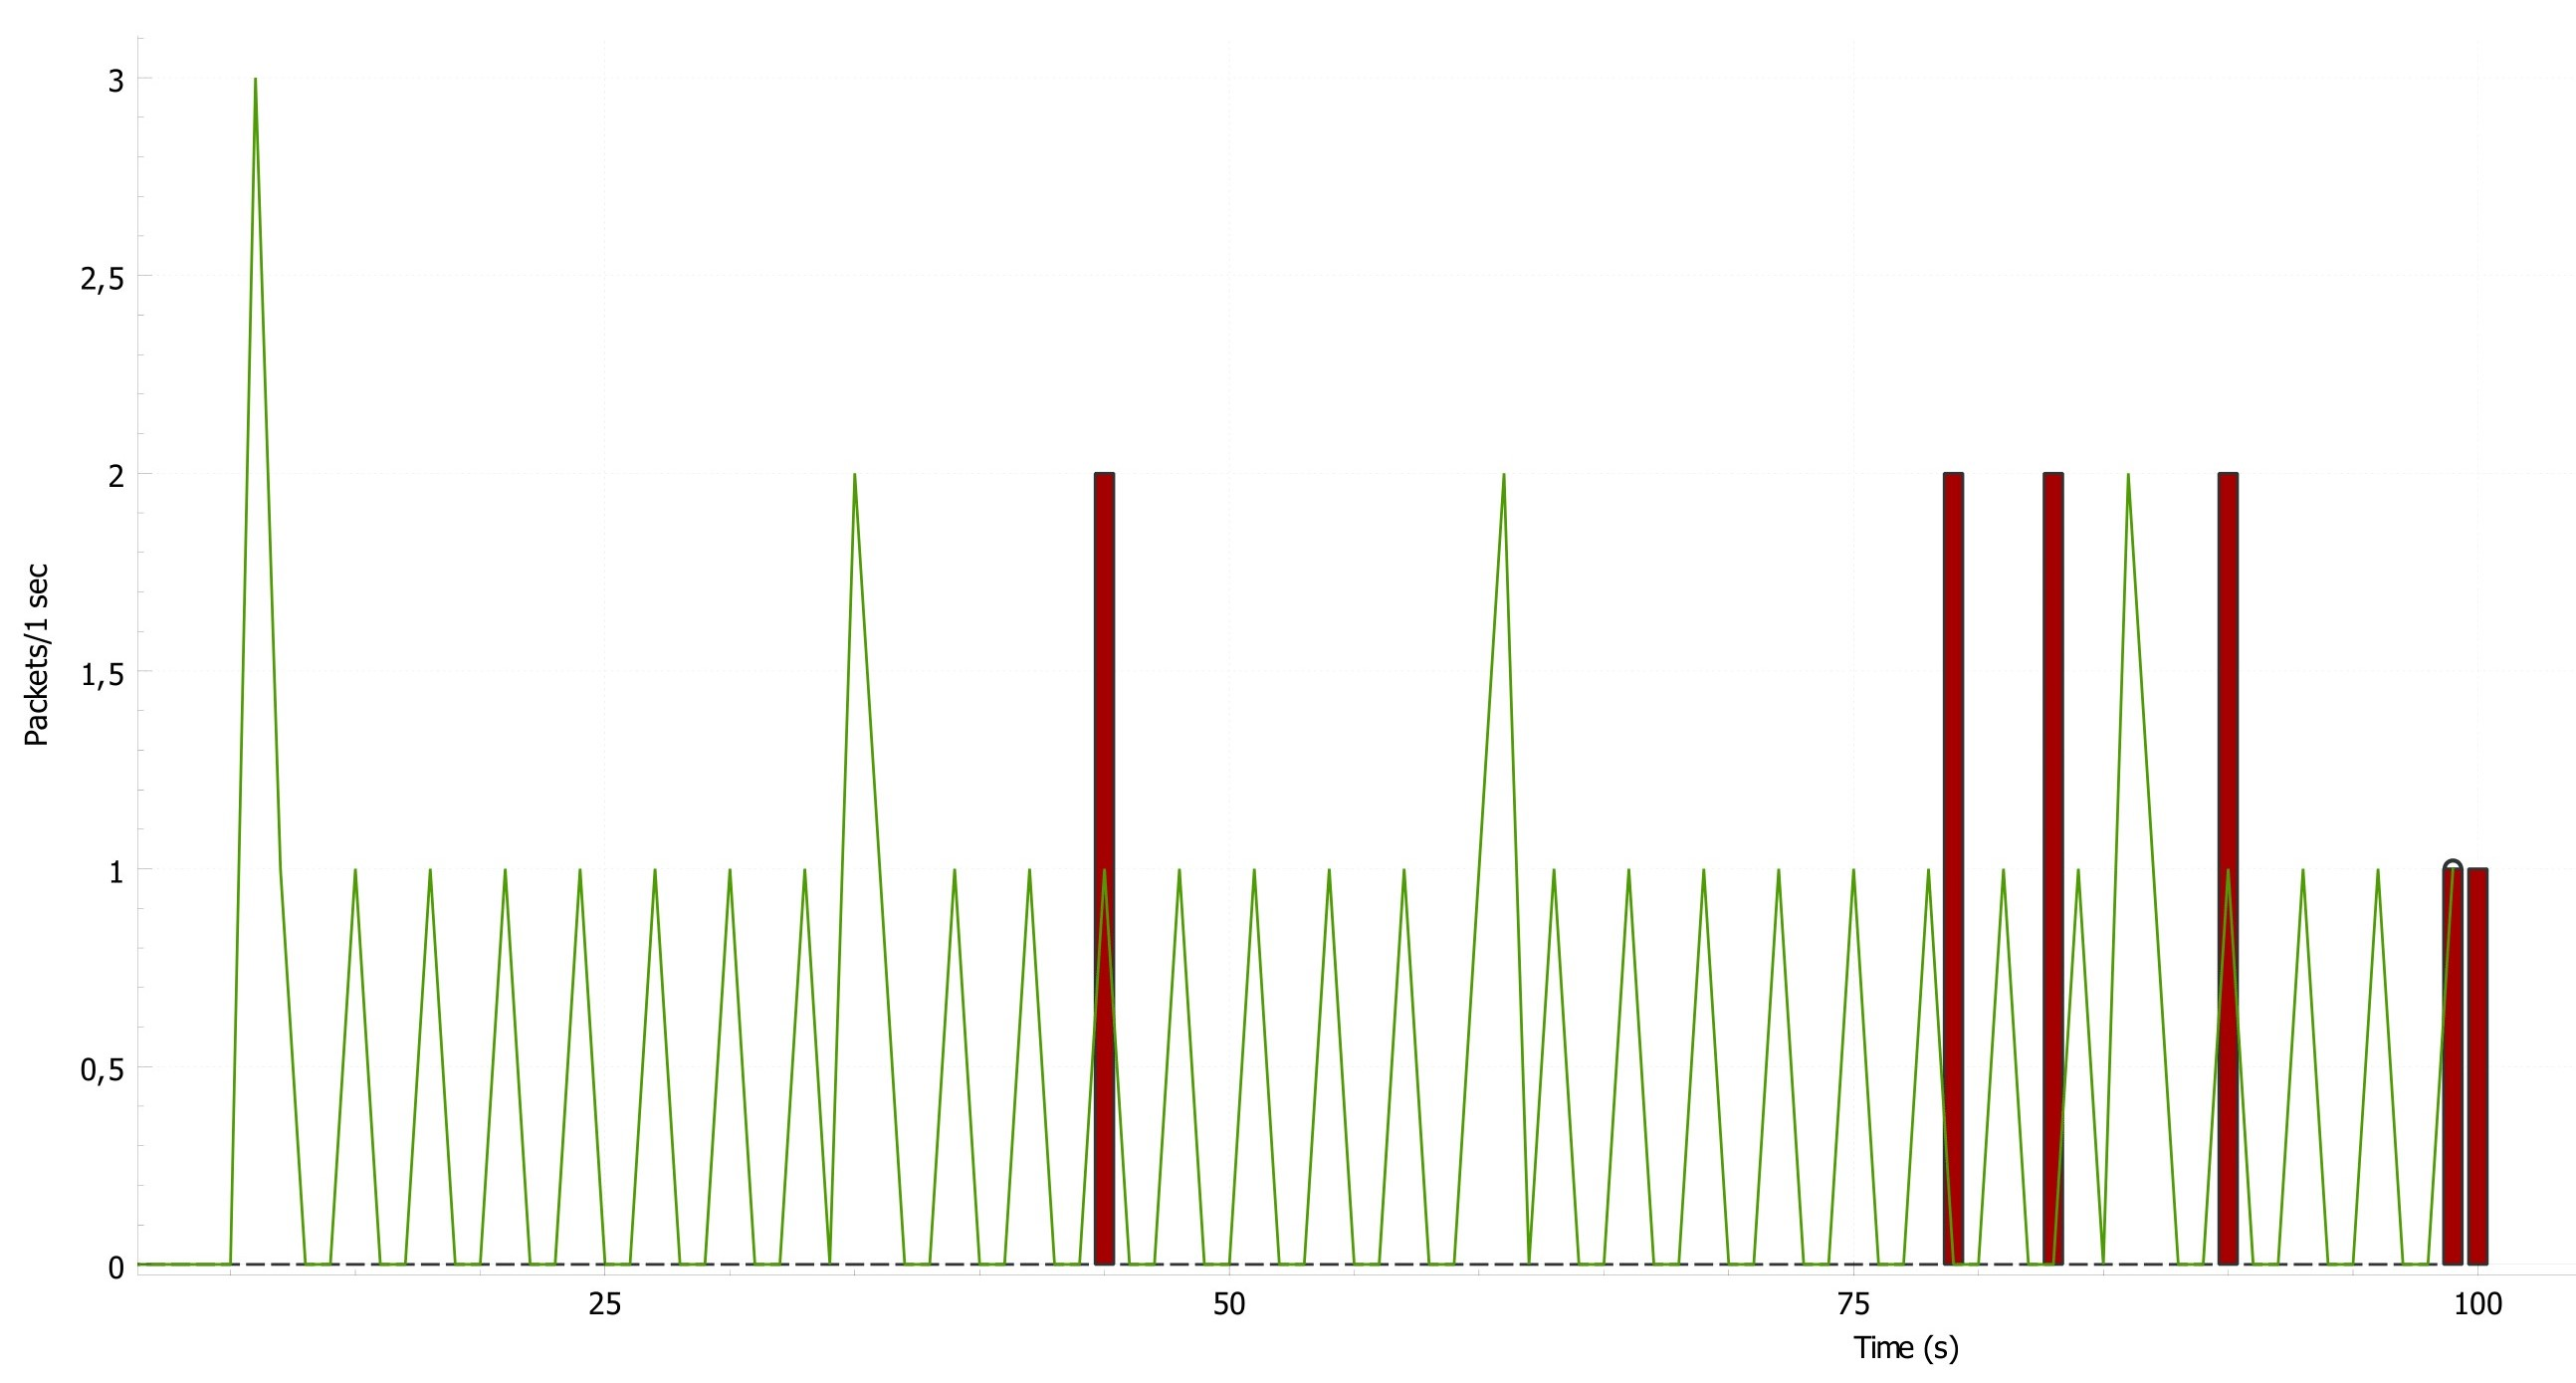
\includegraphics[width=12cm]{websocket traffic hall.jpg}
  \caption{Websocket packet drop collected near the router}
  \label{websocket-traffic-near}
\end{figure}

\begin{figure}[H]
  \centering
  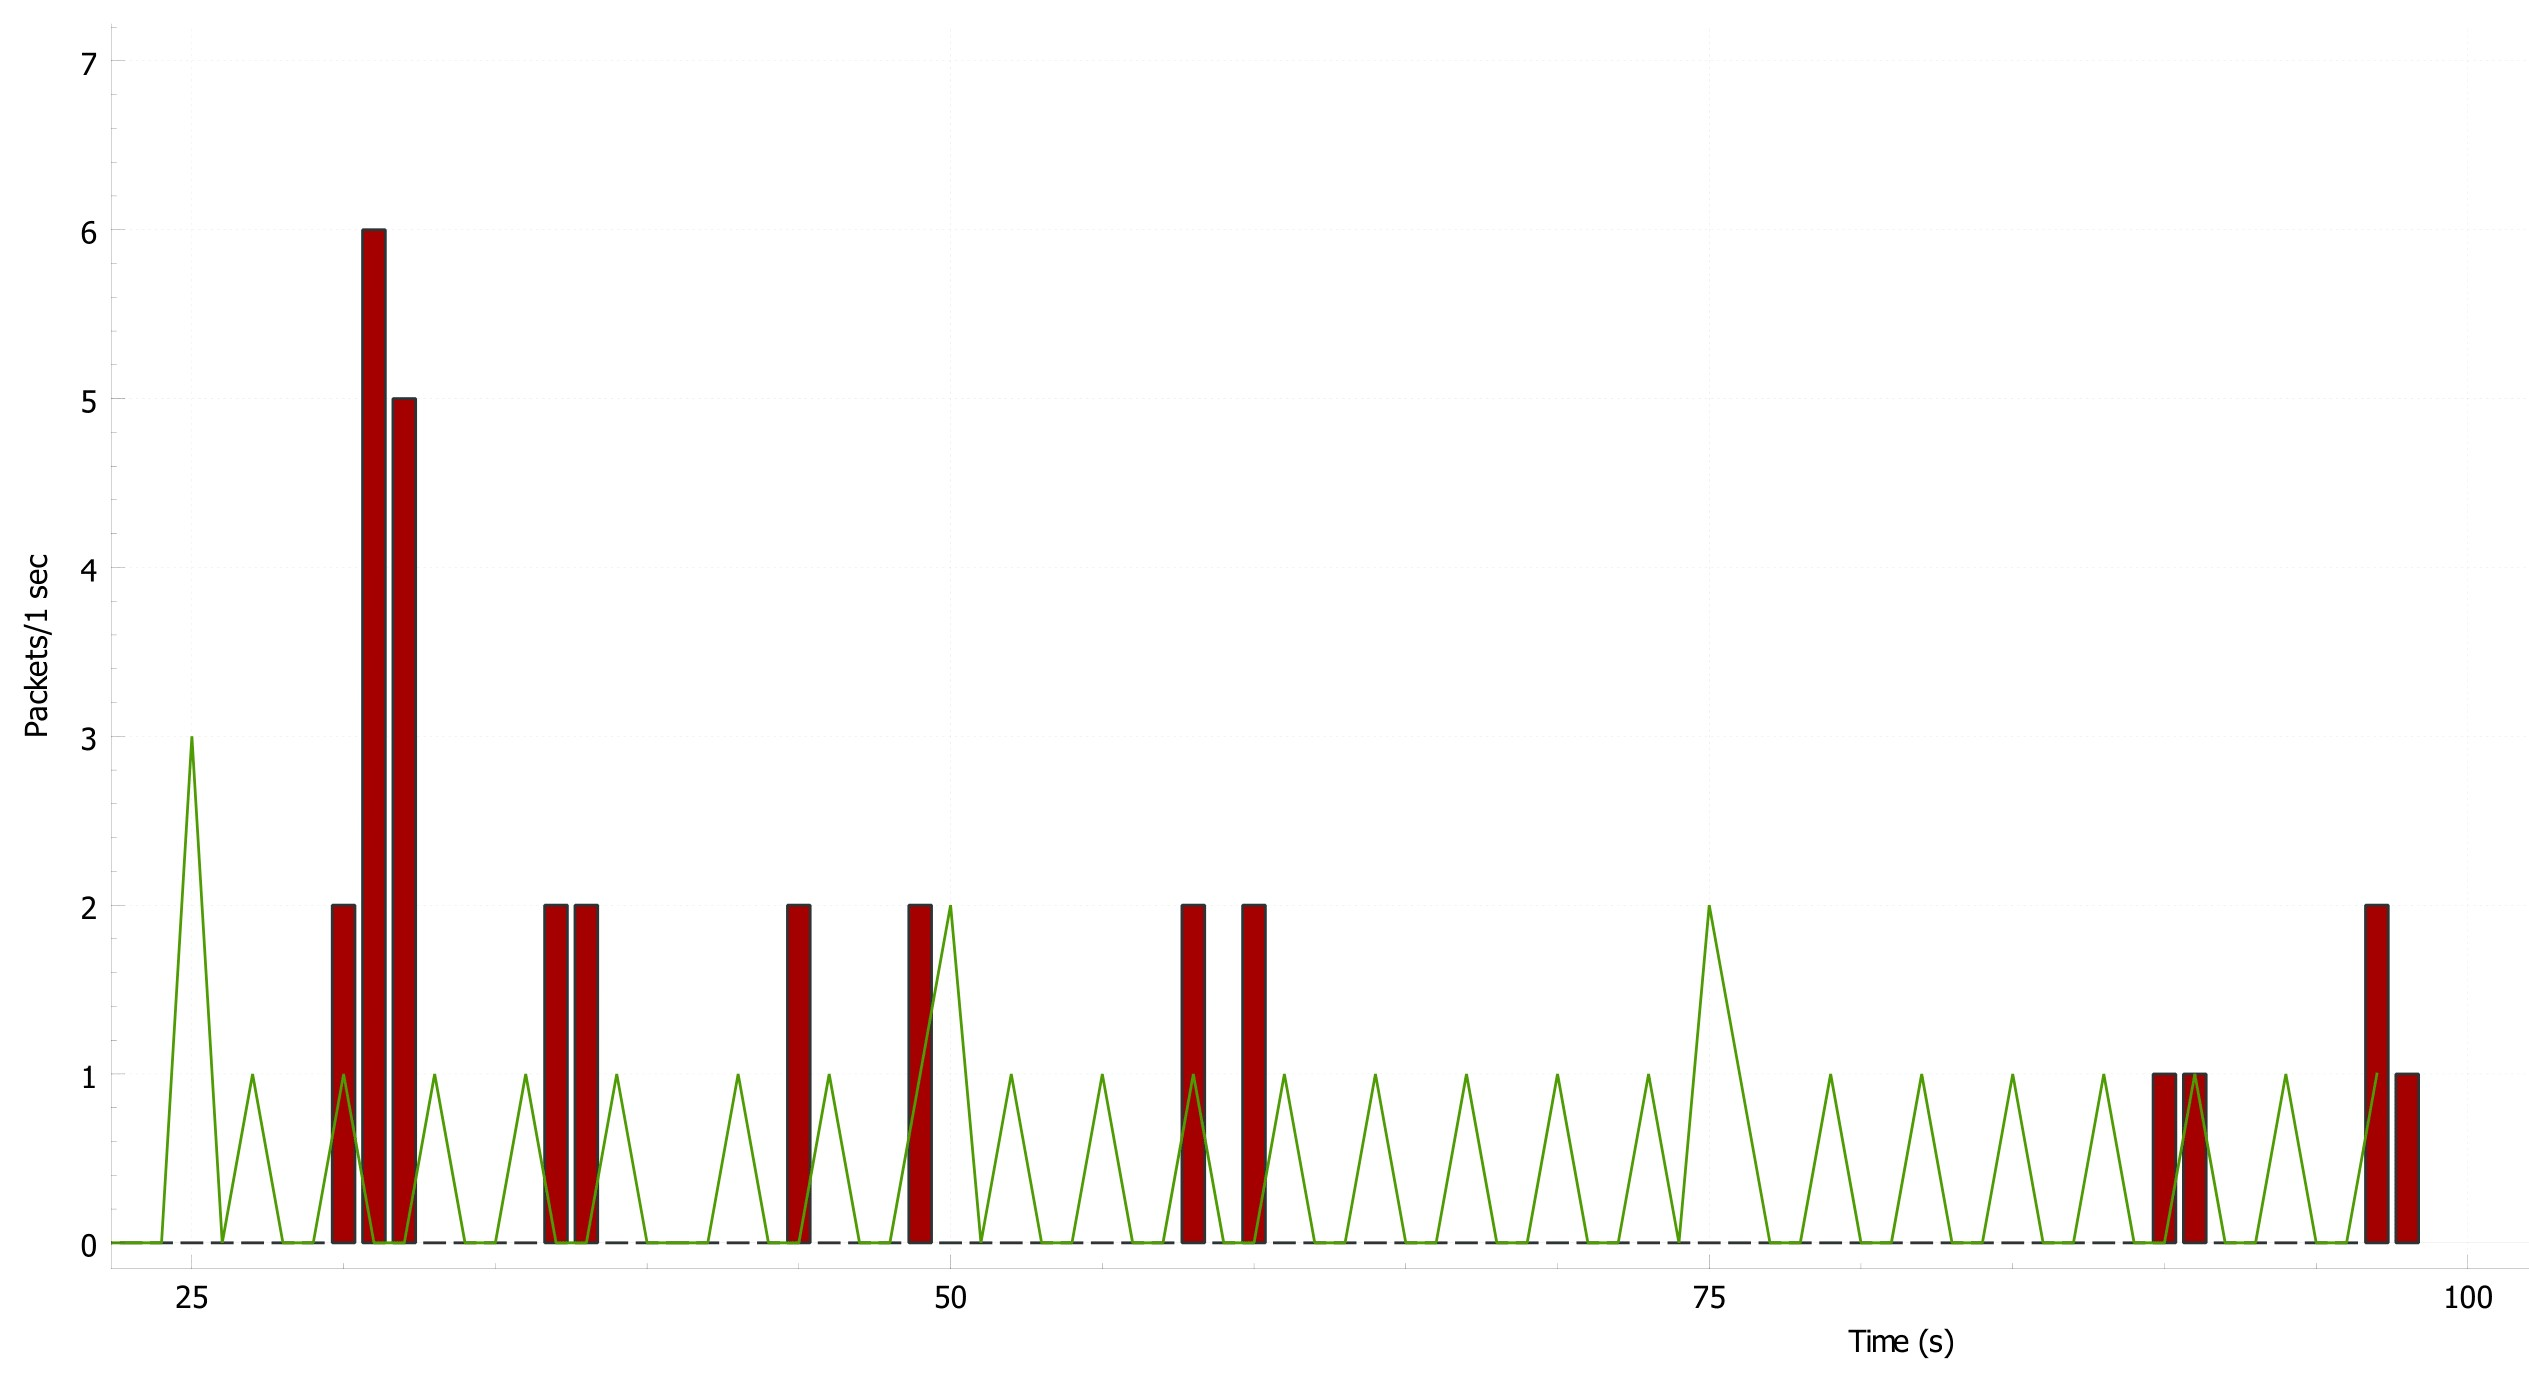
\includegraphics[width=12cm]{websocket traffic bedroom.jpg}
  \caption{Websocket packet drop collected with a door in front of the router}
  \label{websocket-traffic-door}
\end{figure}

The charts above were generated by Wireshark itself, using the green lines to represent
how many packets were successfuly delivered/received through the websocket connection, whereas the
red bars indicate how many packet drops happened during this communication. Notice that there is a significantly
higher flow on the very beginning, which happens due to the bootstrap action described on section III. Meanwhile, at the very end
of both charts, we may see more errors as a consequence of the client disconnection (the browser has been closed). This is the common
behavior in both experiments. However, the charts depict two major different scenarios. The first one, in which the data was collected near
the router, as a way of generating ideal conditions, the packets flow much easier, with a small number of errors. In contrast, the second experiment
depicted a low stability communication, with much frequent packet drops. This behavior was mainly caused by the physical barrier inserted between the pair client/server
and the intermediate router communicating them, making explicit the real conditions faced by such applications, since many similar interferences may occur on regular situations
due to obstables like walls or doors, or even the mobility of the client.

\section{\textbf{Conclusion}}
This paper presented an analysis of the websocket traffic in a simple multiplayer game, collected using the Wireshark tool, in two different situations. The results suggests that including a physical barrier in the communication significantly increases the number of packet drops, since it lowers the stability. Also, the packet drops in the end of the figures~\ref{websocket-traffic-near} and~\ref{websocket-traffic-door} is a consequence of client disconnection, while the high flow in the beginning happens due to bootstrap actions. The authors conclude that websocket connections provide the reliability, robustness and high-performance needed for multiplayer browser-based games, despite of the packet drops presented in section IV.

\bibliography{sbrt}
\bibliographystyle{IEEEtran}

\end{document}
